\providecommand{\topdir}{..}
\documentclass[../main.tex]{subfiles}

\ifSubfilesClassLoaded{
    \externaldocument[main-]{../main}
    \setcounterref{chapter}{main-chap:rayleigh_benard}
    \addtocounter{chapter}{-1}
}{}

\externaldocument{\subfix{../00_front_matter/front_matter}}
\externaldocument{\subfix{../01_introduction/introduction}}
\externaldocument{\subfix{../02_lorenz96/lorenz96}}
\externaldocument{\subfix{../04_tendencies/tendencies}}
\externaldocument{\subfix{../05_evaluation/evaluation}}
\externaldocument{\subfix{../06_conclusion/conclusion}}
\externaldocument{\subfix{../07_appendix/appendix}}

\begin{document}

\ifSubfilesClassLoaded{
    \frontmatter
    \tableofcontents
    \mainmatter
}{}

\dropchapter{4.5cm}
\chapter{\rb{} convection} \label{chap:rayleigh_benard}
\setlength{\epigraphwidth}{0.9\linewidth}
\epigraphhead[0.13\textheight]{
    \epigraph{
        \begin{minipage}{0.52\linewidth}
            Talia flammato secum dea corde volutans \\
            nimborum in patriam, loca feta furentibus austris, \\
            Aeoliam venit. Hic vasto rex Aeolus antro \\
            luctantes ventos tempestatesque sonoras \\
            imperio premit ac vinclis et carcere frenat. \\
            Illi indignantes magno cum murmure montis \\
            circum claustra fremunt; celsa sedet Aeolus arce \\
            sceptra tenens, mollitque animos et temperat iras. \\
            Ni faciat, maria ac terras caelumque profundum \\
            quippe ferant rapidi secum verrantque per auras. \\
            Sed pater omnipotens speluncis abdidit atris, \\
            hoc metuens, molemque et montis insuper altos \\
            imposuit, regemque dedit, qui foedere certo \\
            et premere et laxas sciret dare iussus habenas.
        \end{minipage}
        \hspace{\fill}
        \begin{minipage}{0.45\linewidth}
            Thus inwardly brooding with heart inflamed, the goddess came
            to Aeolia, motherland of storm clouds, tracts teeming with
            furious blasts. Here in his vast cavern, Aeolus, their king,
            keeps under his sway and with prison bonds curbs the
            struggling winds and the roaring gales. They, to the
            mountain's mighty moans, chafe blustering around the
            barriers. In his lofty citadel sits Aeolus, sceptre in hand,
            taming their passions and soothing their rage; did he not
            so, they would surely bear off with them in wild flight seas
            and lands and the vault of heaven, sweeping them through
            space. But, fearful of this, the father omnipotent hid them
            in gloomy caverns, and over them piled high mountain masses
            and gave them a king who, under fixed covenant, should be
            skilled to tighten and loosen the reins at command.
        \end{minipage}
        \vspace{.5\baselineskip}
    }{
        Virgil, \emph{Aeneid I}, ll. 50--63 \\
        trans. H. R. Fairclough
    }
}
\undodrop

Having established a useful set of tools and identified directions for further
work in the previous chapter's review of the Lorenz '96 literature, I now
propose to use two-dimensional \rb{} convection as an intermediate-complexity
test problem for data-driven parametrisation.
\crefrange{sec:rb_equations}{sec:config} first cover the governing equations
and the numerical methods used to solve them.
\cref{sec:resolution,sec:choose_resolution} then take the important step of
choosing the spatial resolutions of the models used for data-driven
parametrisation, first reviewing relevant literature and then performing
numerical experiments.


\section{Governing equations}
\label{sec:rb_equations}
\rb{} convection is the overturning motion of a fluid confined between two
horizontal isothermal plates, the bottom plate being warmer than the top plate.
The fluid is traditionally assumed to be incompressible, with density $\rho$
related to temperature $T$ by the linear equation of state
\[
    \rho = \rho_0 [1 - \alpha(T - T_0)],
\]
$\alpha$ being the volume coefficient of thermal expansion and $\rho_0$ and
$T_0$ a reference density and temperature. Provided that the density variations
are small ($\alpha (T - T_0) \ll 1$), one may employ the \emph{Boussinesq
approximation}, neglecting density variations everywhere except in their
contribution to the weight force. This leads to the Boussinesq equations
\begin{align}
    \label{eqn:dim_momentum}
    \pdiff{\vec{u}}{t} + \vec{u} \cdot \grad \vec{u}
        &= -\frac{1}{\rho_0} \grad p' + \alpha (T - T_0) g \uvec{z}
            + \nu \nabla^2 \vec{u}, \\
    \label{eqn:dim_energy}
    \pdiff{T}{t} + \vec{u} \cdot \grad T &= \kappa \nabla^2 T,
        \quad \text{and} \\
    \label{eqn:dim_incompressible}
    \grad \cdot \vec{u} &= 0,
\end{align}
which represent the momentum balance, the conservation of energy and the
assumption of incompressiblity, respectively. The prognostic variables are the
fluid velocity $\vec{u}$ and the temperature $T$ (the pressure perturbation
$p'$ is implicitly determined by \cref{eqn:dim_incompressible}). The parameters
of the model are the kinematic viscosity $\nu$ and thermal diffusivity
$\kappa$. $\uvec{z}$ is the upward unit vector. The Boussinesq approximation
has led to the appearance of a buoyant force (per unit mass)
\[
    \alpha (T - T_0) g = \frac{\rho_0 - \rho}{\rho_0} g
\]
in the momentum equation, in agreement with Archimedes' principle. The reader
is referred to \textcite{chandrasekhar1961} for a detailed derivation of the
Boussinesq equations; I have merely summarised the main assumptions and
approximations involved.

In this work, I consider solutions of
\crefrange{eqn:dim_momentum}{eqn:dim_incompressible} in a two-dimensional
domain $[0, d] \times [0, L]$ with Cartesian coordinates $x$ and $z$, subject
to no-slip, isothermal boundary conditions
\begin{alignat}{3}
    \label{eqn:dim_bc_bot}
    \vec{u} &= \vec{0}, &\quad T &= T_0 + \frac{\delta T}{2} &\quad& \text{at
    } z = 0 \text{ and} \\
    \label{eqn:dim_bc_top}
    \vec{u} &= \vec{0}, &\quad T &= T_0 - \frac{\delta T}{2} &\quad& \text{at
    } z = d
\end{alignat}
on the top and bottom plates, and periodic boundary conditions
\begin{alignat}{2}
    \label{eqn:dim_bc_sides}
    \vec{u}(x=0) &= \vec{u}(x=L) &\quad \text{and} \quad T(x=0) &= T(x=L)
\end{alignat}
in the horizontal. $\delta T$ is the constant temperature difference between
the plates.

\section{Nondimensionalisation and scale analysis}
It is helpful to nondimensionalise the governing equations
\crefrange{eqn:dim_momentum}{eqn:dim_bc_sides}; this is not only useful for
numerical work but also gives insight into the different flow regimes that are
possible. A range of nondimensionalisations are used in fluid dynamics
literature; I adopt a common one \parencite[see,
e.g.,][]{grotzbach1983,ouertatani2008,stevens2010} which is suitable for the
turbulent convective regime.

The first step is to choose representative time, length and temperature scales.
For low-viscosity, turbulent flow, a suitable time scale is the \emph{free-fall
time} $t_0$, which is the time for a fluid element with constant temperature $T
= T_0 - \delta T$ to fall from the top plate to the bottom plate under the
influence of buoyancy ($-g \alpha \delta T$) alone. It is simple to show that
\[
    t_0 \sim \left( \frac{d}{g \alpha \delta T} \right)^{1/2},
\]
ignoring a factor of $\sqrt{2}$. The obvious length and temperature scales are
the plate separation $d$ and temperature difference $\delta T$, respectively.

Making the substitutions $p'/\rho_0 \to \pi$ and $T - T_0 \to \theta$ in
\crefrange{eqn:dim_momentum}{eqn:dim_bc_sides} and expressing all variables in
units of $t_0$, $d$ and $\delta T$ leads to the dimensionless equations
\begin{align}
    \label{eqn:momentum}
    \pdiff{\vec{u}}{t} + \vec{u} \cdot \grad \vec{u}
        &= -\grad \pi + \left( \frac{\prandtl}{\rayleigh}\right)^{1/2}
        \nabla^2 \vec{u} + \theta \uvec{z}, \\
    \label{eqn:energy}
    \pdiff{\theta}{t} + \vec{u} \cdot \grad \theta
        &= (\rayleigh\,\prandtl)^{-1/2} \, \nabla^2 \theta, \quad \text{and} \\
    \label{eqn:incompressible}
    \grad \cdot \vec{u} &= 0,
\end{align}
which are solved in the domain $[0, \Gamma] \times [0, 1]$ with boundary
conditions
\begin{gather}
\begin{alignat}{3}
    \label{eqn:bc_bot}
    \vec{u} &= \vec{0}, &\quad \theta &= +\frac{1}{2}
    &\qquad& \text{at } z = 0, \\
    \label{eqn:bc_top}
    \vec{u} &= \vec{0}, &\quad \theta &= -\frac{1}{2}
    &\qquad& \text{at } z = 1,
\end{alignat} \\
\begin{alignat}{2}
    \label{eqn:bc_sides}
    \vec{u}(x=0) &= \vec{u}(x=\Gamma)
    &\quad \text{and} \quad \theta(x=0) &= \theta(x=\Gamma).
\end{alignat}
\end{gather}
There are three dimensionless parameters: the aspect ratio of the domain
\[
    \Gamma \equiv \frac{L}{d},
\]
the \emph{Prandtl number}
\[
    \prandtl \equiv \frac{\nu}{\kappa}
\]
which measures the relative importance of viscosity (momentum diffusivity) and
thermal diffusivity, and the \emph{Rayleigh number}
\[
    \rayleigh \equiv \frac{g \alpha d^3 \delta T}{\kappa \nu}.
\]
The Rayleigh number can be interpreted as the ratio of the time scale for
thermal transport by conduction to the time scale for thermal transport by
convection. It determines the importance of diffusion for the evolution of
$\vec{u}$ and $\theta$; inspection of \cref{eqn:momentum,eqn:energy} indicates
that low $\rayleigh$ implies strong diffusion and high $\rayleigh$ weak
diffusion. Stability analysis (see, e.g., \textcite{chandrasekhar1961} and the
seminal work by \textcite{rayleigh1916}) reveals that there exists a critical
Rayleigh number (dependent on boundary conditions but of order $\SI{e3}{}$),
below which the equations have a stable equilibrium with the fluid at rest and
a linear conductive temperature profile. Above the critical Rayleigh number,
the equilibrium is unstable and small perturbations lead to the formation of a
regular series of steady convection cells. If the Rayleigh number is increased
much further (\textcite{le_quere1991} cites $\rayleigh \approx \SI{2e8}{}$),
the solution becomes unsteady and increasingly turbulent. This work is
concerned with the turbulent regime, since Rayleigh numbers for atmospheric
deep moist convection can be as large as $\SI{e22}{}$ \parencite{chilla2012}.


\section{Hyperdiffusion terms} \label{sec:hyper}
In \cref{chap:evaluation} I will compare the output of a parametrised
low-resolution model of \crefrange{eqn:dim_momentum}{eqn:bc_sides} to the
output of the unparametrised base model (i.e., the control). However, it was
found in the early stages of this work that unparametrised low-resolution
models were prone to numerical instability, preventing the obtainment of a
suitable control solution. This is to be expected; at high Rayleigh numbers,
when dissipation is weak, the solutions develop large gradients near
small-scale features that cannot be properly resolved by coarse models, causing
the model to crash. To be more precise, the energy spectra of turbulent flows
exhibit an \emph{energy cascade} whereby energy is transferred from
larger-scale motions to smaller-scale motions; only at sufficiently small
scales is energy removed from the system by the dissipative terms in the
equations \parencite{pope2000}. In coarse models where these smallest scales
are not resolved, excess energy accumulates at the highest resolved
wavenumbers.

I choose to stabilise the numerical model by introducing artificial dissipative
terms that act on the smallest scales. The modified equations, with the new
terms highlighted in red, are
\begin{align}
    \label{eqn:hyper_momentum}
    \pdiff{\vec{u}}{t} + \vec{u} \cdot \grad \vec{u}
        &= -\grad \pi + \left( \frac{\prandtl}{\rayleigh}\right)^{1/2}
            \left(
                \nabla^2 \vec{u} + {\color{red}
                \tilde{\nu} f(z) |\nabla^2 \vec{u}| \nabla^2 \vec{u}}
            \right)
            + \theta \uvec{z}, \\
    \label{eqn:hyper_energy}
    \pdiff{\theta}{t} + \vec{u} \cdot \grad \theta
        &= (\rayleigh\,\prandtl)^{-1/2}
            \left(
                \nabla^2 \theta + {\color{red}
                \tilde{\kappa} f(z) |\nabla^2 \theta| \nabla^2 \theta}
            \right), \quad \text{and} \\
    \label{eqn:hyper_incompressible}
    \grad \cdot \vec{u} &= 0,
\end{align}
where the constants $\tilde{\nu} = \tilde{\kappa} = \SI{2e-3}{}$ were chosen by
trial and error to achieve sufficient dissipation. The function $f(z)$ is
necessary to reduce the artificial terms to zero near the top and bottom of the
domain (otherwise the model crashes) while leaving them relatively unchanged
in the interior, and is defined by
\[
    f(z) = \left[
        1 - \exp \left( -\frac{\min(z, 1-z)}{0.052} \right)
    \right]^4.
\]
The definition of $f(z)$ is inspired by the \emph{van Driest damping function}
commonly used in large-eddy simulations of wall-bounded flows
\parencite{pope2000}.

The new additions are akin to regular viscous and diffusive terms with
viscosity and diffusivity coefficients that depend on second derivatives of the
flow variables. Small-scale features, where $|\nabla^2 \vec{u}|$ and/or
$|\nabla^2 \theta|$ are large, will experience a larger effective viscosity
and/or thermal diffusivity respectively, and therefore be dissipated more
rapidly than larger-scale features.

It must be emphasised that this work is \emph{not} concerned with whether or
not these modified equations are an accurate representation of physical
reality; they simply serve as an example dynamical system for the study of
parametrisation.


\section{Model configuration}
\label{sec:config}
The nondimensionalised Boussinesq equations
\crefrange{eqn:hyper_momentum}{eqn:hyper_incompressible} and
\crefrange{eqn:bc_bot}{eqn:bc_sides} are solved numerically using Dedalus
(\texttt{v3}), a spectral code built in Python \parencite{burns2020}. Spectral
methods represent the solution of a partial differential equation as a linear
combination of linearly independent basis functions, solving for the
coefficients of the basis function expansion rather than the values of the
solution in real space. The resolution of the model is thus set by choosing the
number of basis functions used. This work uses a Fourier (sine/cosine) basis in
the horizontal direction and a basis of Chebyshev polynomials (of the first
kind) in the vertical direction. The Fourier basis has the special property
that all linear combinations respect the periodic boundary conditions.
For storage and analysis, the model output is transformed into real space,
where the fields are defined on a \emph{collocation grid} that is has uniform
horizontal spacing but non-uniform vertical spacing (smaller near the top and
bottom of the domain and larger in the middle).

Timestepping is performed using a second-order Runge-Kutta scheme. The Rayleigh
number was set to $10^9$, a value at which the flow was found to be unsteady
and feature transient eddies. The aspect ratio of the domain was $\Gamma = 8$
and the Prandtl number was set to $1$ for simplicity. The complete model source
code is publicly available; see \cref{chap:computations}.


\section{Choice of resolution: literature} \label{sec:resolution} The next
important step is to choose the resolution of the fine and coarse models that
will be used in the data-driven parametrisation process. The fine model will
serve as ``truth'', providing the training dataset to which the parametrisation
model will be fitted and the test dataset against which the parametrised coarse
model will be evaluated. Its resolution should therefore be high enough that
the (yet-to-be-)chosen evaluation metrics are relatively insensitive to small
changes in resolution (i.e., there should be near-convergence of long-term
statistics). Note, however, that neither a perfect solution of the fluid
equations nor perfect agreement with real-world experimental measurements are
necessary; the fine model merely serves as a reference dynamical system whose
behaviour I aim to reproduce by parametrising the coarse model. In order to
create a worthwhile parametrisation problem, the coarse model's resolution
should therefore be low enough that it exhibits statistically significant
biases relative to the fine model, as measured by the chosen evaluation
metrics. However, as explained in \cref{sec:hyper}, the coarse model must still
be numerically stable so that it can provide an unparametrised control
solution.

With the above constraints in mind, \cref{sec:res_requirements} will review the
guidelines that have been established in the literature for producing
well-resolved simulations of \rb{} convection. \cref{sec:metrics} will
then review the metrics that are known to be sensitive to under-resolution;
these may be used to experimentally determine appropriate resolutions for the
fine and coarse models, and later (in \cref{chap:evaluation}) to evaluate
parametrisation performance.


\subsection{Resolution guidelines}
\label{sec:res_requirements}

\textcite{grotzbach1983} is recognised as the first to formulate resolution
requirements for accurate simulations of \rb{} convection
\parencite{chilla2012,scheel2013}. He identified separate constraints on the
mean (i.e., averaged in each spatial direction) grid spacing and the vertical
spacing near the plates; I first discuss the former. \citeauthor{grotzbach1983}
reasoned that a numerical model that neglects subgrid-scale effects must have a
geometric mean grid spacing $h$ (i.e. $h = (\Delta x \Delta y \Delta z)^{1/3}$
in 3D) such that
\begin{equation}
    \label{eqn:grotzbach}
    h \leq \pi \underbrace{
        \left( \frac{\prandtl}{\rayleigh} \right)^{3/8}
        \langle \epsilon_k \rangle^{-1/4}
    }_{\eta},
\end{equation}
where $\eta$ is the \emph{Kolmogorov length}, the universal smallest relevant
length scale for general turbulent flow, and $\langle \epsilon_k \rangle$ is
the spatial and temporal average of the kinetic energy dissipation rate defined
by
\begin{equation}
    \label{eqn:kinetic_dissipation}
    \epsilon_k(\vec{x}, t) \equiv
        \frac{1}{2} \left( \frac{\prandtl}{\rayleigh} \right)^{1/2}
        \sum_{ij} \left( \pdiff{u_i}{x_j} + \pdiff{u_j}{x_i} \right)^2
\end{equation}
\parencite{chilla2012}. The inequality \cref{eqn:grotzbach} between $h$ and
$\eta$ can be understood using the Nyquist-Shannon theorem, which states that a
sampling frequency $f \geq k/\pi$ is needed to unambiguously reconstruct a
signal with maximum wavenumber $k$; substituting $f = 1/h$, $k = 1/\eta$ leads
to the claimed relation.

\citeauthor{grotzbach1983} recognised that the above reasoning was only valid
for the mean grid spacing; large gradients in temperature and velocity near the
top and bottom plates require finer resolution in those regions. The notion of
nearness can be formalised by considering the thickness of the \emph{thermal
boundary layer}, the region at each plate where large temperature gradients
exist. Consider a Taylor series expansion of the horizontally- and
time-averaged dimensionless temperature profile about $z=0$; recalling the
boundary condition \cref{eqn:bc_bot}, this reads
\[
    \langle \theta \rangle _{A,t} \approx \frac{1}{2}
        + \left. \pdiff{\langle \theta \rangle _{A,t}}{z} \right|_{z=0} z
        + O(z^2).
\]
The thermal boundary layer thickness $\delta_\theta$ is defined \parencite[see,
e.g.,][]{chilla2012} as the height at which, to first order, the temperature
reaches the mean value in the well-mixed interior of the domain (i.e., zero for
this problem). It follows that
\begin{equation}
    \label{eqn:thermal_bl}
    \delta_\theta = -\frac{1}{2} \left(
        \left. \pdiff{\langle \theta \rangle _{A,t}}{z} \right|_{z=0}
    \right)^{-1}.
\end{equation}

And similarly for the other boundary layer at $z=1$. One then asks how many
grid points must be within the thermal boundary layer.
\citeauthor{grotzbach1983} claimed that 3 points are sufficient for turbulent
flows but did not give a theoretical argument to derive this number.
\textcite{shishkina2010} presented a theoretical argument based on the
(experimentally and numerically justified) assumption of laminar
\emph{Prandtl-Blasius} flow conditions in the boundary layer and were able to
calculate the minimum number of grid points (e.g., 9 for $\rayleigh =
\SI{2e9}{}$ and $\prandtl = 0.7$). The results agreed with criteria derived in
previous numerical experiments. Importantly, the results of
\citeauthor{shishkina2010} allow \emph{a priori} determination of vertical
resolution requirements, potentially bypassing the time-consuming and expensive
process of iteratively running simulations, checking their convergence and
updating the resolution.


\subsection{Metrics sensitive to under-resolution} \label{sec:metrics}
Performing numerical experiments for a 3D fluid layer,
\citeauthor{grotzbach1983} found that the RMS velocity and the \emph{Nusselt
number} were the most sensitive quantities to insufficient mean grid spacing,
but even they increased ``only slightly'' above the values obtained from
well-resolved simulations. The dimensionless Nusselt number measures the
instantaneous rate of (vertical) heat transport across a horizontal plane at
height $z$, normalised by the purely conductive rate that would exist if the
fluid were at rest \parencite{verzicco1999}. Following \textcite{kooij2018}, I
define
\[
    \nusselt(z,t) \equiv \sqrt{\rayleigh\,\prandtl} \langle w \theta \rangle _A
        - \left\langle \pdiff{\theta}{z} \right\rangle _A
\]
where $\langle \cdot \rangle _A$ denotes averaging over the horizontal plane at
height $z$, and $w = \vec{u} \cdot \uvec{z}$ is the vertical velocity. Notice
that the heat transport has contribitions from both advection (the first term)
and conduction (the second term). Authors frequently consider the
vertically-averaged value
\begin{equation} \label{eqn:nusselt_zavg}
    \langle \nusselt(z,t) \rangle _z
        = \sqrt{\rayleigh\,\prandtl} \langle w \theta \rangle _{A,z} + 1
\end{equation}
and/or the time-averaged value, which is is independent of height due to
energy conservation,
\[
    \langle \nusselt(z,t) \rangle _t = \langle \nusselt(z,t) \rangle _{z,t}
        = \sqrt{\rayleigh\,\prandtl} \langle w \theta \rangle _{A,z,t} + 1.
\]

Later work also supports the finding that the Nusselt number is sensitive to
under-resolution. Even studying only steady-state convective solutions at
moderate Rayleigh number, \textcite{le_quere1991} found that the maximum and
minimum Nusselt numbers were most sensitive to changes in resolution and had
the largest uncertainty among existing benchmark solutions.
Other studies have used the convergence of the Nusselt number as an indicator
that the spatial resolution is sufficient to produce an accurate solution
\parencite{ouertatani2008}.

\textcite{stevens2010} performed 3D simulations in a finite cylindrical cavity
with the aim of reconciling the apparent disagreement between the Nusselt
numbers in previous numerical studies and experimental observations. They found
that agreement with experiment could be achieved, but only by using a much
higher resolution than the previous studies. They offered the physical
explanation that horizontally under-resolved simulations produce insufficient
thermal diffusion, leading to systematic overestimation of the buoyancy of
convective plumes near the side-walls of the cylinder; this results in Nusselt
numbers that exceed experimentally observed values. This led them to conclude
that the two criteria of \textcite{grotzbach1983}---for mean grid spacing and
for the vertical spacing near the upper and lower plates---are not independent;
the definition $h = (\Delta x \Delta y \Delta z)^{1/3}$ in \cref{eqn:grotzbach}
allows the horizontal spacing to remain relatively coarse near the plates,
provided the vertical spacing is small. Since fine horizontal resolution is
also necessary to accurately capture the dynamics of the thin plumes, they
proposed that \cref{eqn:grotzbach} be applied with $h = \max(\Delta x, \Delta
y, \Delta z)$ instead.

Some more recent work, however, casts doubt on the notion that the Nusselt
number is sensitive to under-resolution and that its convergence is a good
indicator that the flow is well-resolved. In assessing the performance of
several published computational fluid dynamics codes on the \rb{} problem in a
cylindrical cavity, \textcite{kooij2018} identified one higher-order code that
reproduced the theoretically predicted scaling of $\nusselt$ as a function of
$\rayleigh$ even when the flow was deliberately under-resolved. On the other
hand, the presence of numerical artefacts in the instantaneous temperature
field near the bottom plate was a clear indicator of insufficient resolution.

\textcite{scheel2013} performed similar high-resolution simulations for a
cylindrical cavity and also found that the Nusselt number, among other global
transport properties, were ``fairly insensitive to insufficient resolution, as
long as the mean Kolmogorov length [was] resolved'' (i.e., \cref{eqn:grotzbach}
was satisfied). However, they found that the horizontally averaged or local
kinetic energy dissipation rate \cref{eqn:kinetic_dissipation} and the
corresponding thermal dissipation rate
\begin{equation}
    \label{eqn:thermal_dissipation}
    \epsilon_\theta(\vec{x}, t) \equiv
        (\rayleigh\,\prandtl)^{-1/2} \sum_i \left(\pdiff{\theta}{x_i}\right)^2
\end{equation}
were much more sensitive, with their convergence requiring even stricter
conditions than \cref{eqn:grotzbach}.


\section{Choice of resolution: experiment} \label{sec:choose_resolution}
I have performed a series of simulations at different resolutions using the
numerical model described in \cref{sec:config}, using the metrics identified in
\cref{sec:metrics} to determine appropriate resolutions for the fine and coarse
models in the parametrisation study of
\cref{chap:tendencies,chap:evaluation}. The coarsest simulation had a
resolution of 256 horizontal (Fourier) modes by 64 vertical (Chebyshev) modes
and the highest 2048 by 256.

Higher-resolution simulations require shorter time steps in order to be stable.
The suitability of the time step is determined by the \emph{Courant number}
\parencite{pope2000}
\[
    C \equiv \frac{|u|}{\Delta x / \Delta t} + \frac{|w|}{\Delta z / \Delta t},
\]
which expresses the horizontal and vertical velocities $u$ and $w$ in units of
the grid spacings\footnote{Since the model uses a spectral method, $\Delta x$
and $\Delta z$ are taken to be the local spacings of the collocation grid in
real space; see \cref{sec:config}.} $\Delta x$ and $\Delta z$ per time step
$\Delta t$, and must be sufficiently small (typically less than 1). The time
step was tuned by trial and error at an intermediate starting resolution (not
shown) and the time step for other resolutions was scaled to approximately
preserve $C$. The scaling is derived by reasoning that, if $|u|$ and $|w|$ are
approximately equal on average and independent of resolution, then for two
simulations denoted by subscripts 1 and 2, the equality of $C_1$ and $C_2$
implies
\begin{align*}
    \frac{1}{\Delta x_1 / \Delta t_1} + \frac{1}{\Delta z_1 / \Delta t_1}
        &= \frac{1}{\Delta x_2 / \Delta t_2}
            + \frac{1}{\Delta z_2 / \Delta t_2} \\
    \Leftrightarrow \qquad
    \Delta t_2
        &= \frac{1/\Delta x_1 + 1/\Delta z_1}{1/\Delta x_2 + 1/\Delta z_2}
            \Delta t_1.
\end{align*}
Recognising that the grid spacings are related to the numbers
of grid points (or spectral modes) $N_x$ and $N_z$ by $\Delta x = \Gamma/N_x$
and $\Delta z \approx 1/N_z$ (where $\Gamma$ is the aspect ratio of the
domain), this may be further simplified to
\[
    \Delta t_2
        = \frac{N_{x_1}/\Gamma + N_{z_1}}{N_{x_2}/\Gamma + N_{z_2}} \Delta t_1.
\]
\cref{tab:resolution_tests} summarises the resolutions of the simulations
and their time steps.

\begin{table}[ht]
\centering
\begin{tabular}{l l l}
    \toprule
    $N_x$ & $N_z$ & $\Delta t$ \\
    \midrule
    256 & 64 & $\SI{5.333e-3}{}$ \\
    512 & 64 & $\SI{4e-3}{}$ \\
    768 & 96 & $\SI{2.667e-3}{}$ \\
    1024 & 128 & $\SI{2e-3}{}$ \\
    1280 & 160 & $\SI{1.6e-3}{}$ \\
    1536 & 192 & $\SI{1.333e-3}{}$ \\
    1792 & 224 & $\SI{1.143e-3}{}$ \\
    2048 & 256 & $\SI{1e-3}{}$ \\
    \bottomrule
\end{tabular}
\caption{
    Resolutions and time steps of the simulations used in the
    resolution-dependence experiment.
}
\label{tab:resolution_tests}
\end{table}

The simulations with resolution $1024 \times 128$ and coarser were started from
the initial condition described in \cref{sec:initial_condition} and run for
1000 time units. The simulations with resolution finer than $1024 \times 128$
were initialised by interpolating the $1024 \times 128$ solution at time $t =
650$ and run for a further 350 time units to reduce computational cost. All
output was saved at an interval of approximately 0.2 time units. The first 750
time units of data were discarded to ensure that all simulations had reached a
statistically steady state (\cref{sec:spinup} verifies this).

For each simulation, I calculated time averages of the following quantities:
\begin{enumerate}[a.]
    \item The vertically-averaged Nusselt number
        $\langle \nusselt(z,t) \rangle _z$, defined by \cref{eqn:nusselt_zavg},
    \item The horizontally-averaged thickness of the two thermal boundary
        layers $( \langle \delta_{\theta, z=0} \rangle _x
        + \langle \delta_{\theta, z=1} \rangle _x )/2$, defined by
        \cref{eqn:thermal_bl},
    \item The RMS speed $\sqrt{\langle \vec{u} \cdot \vec{u} \rangle _{x,z}}$,
    \item The domain-averaged kinetic energy dissipation rate $\langle
        \epsilon_k \rangle _{x,z}$, defined by \cref{eqn:kinetic_dissipation},
        and
    \item The domain-averaged thermal dissipation rate $\langle \epsilon_\theta
        \rangle _{x,z}$, defined by \cref{eqn:thermal_dissipation}.
\end{enumerate}

Time averaging was performed over the 250 time units of data that remained
after discarding the first 750. I identified two related dominant sources of
uncertainty in the calculated values: (i) the uncertainty due to the finite
averaging time and (ii) the uncertainty arising from low-frequency fluctuations
of the quantities being averaged (i.e., the fact that the results change if the
finite averaging window is translated in time). I estimated (i) as half the
range of the running mean,
\begin{equation} \label{eqn:running_mean}
    \frac{1}{2} ~ \underset{\tau \in [150, 250]}{\operatorname{range}} ~
        \frac{1}{\tau} \int_{750}^{750 + \tau} (\cdot) ~\d{t},
\end{equation}
which measures the sensitivity of the result to changes in the averaging time.
I estimated (ii) as half the range of the 150-time-unit rolling mean,
\begin{equation} \label{eqn:rolling_mean}
    \frac{1}{2} ~ \underset{\tau \in [0, 100]}{\operatorname{range}} ~
        \frac{1}{150} \int_{750 + \tau}^{900 + \tau} (\cdot) ~\d{t},
\end{equation}
which measures the sensitivity of the result to the translation of the
averaging window. I took the larger of \cref{eqn:running_mean,eqn:rolling_mean}
as a conservative estimate of the overall uncertainty.

\cref{fig:resolution_dependence} shows plots of the five metrics as functions
of resolution, expressing the values as percentage errors relative to the
highest-resolution simulation. Firstly, observe that all the metrics (except
perhaps the RMS speed) appear insensitive to small changes in resolution about
$2048 \times 256$; I therefore choose $2048 \times 256$ as the resolution of the
fine ``truth'' model for the parametrisation study.

All five metrics exhibit statistically significant discrepancies across the
range of resolutions tested. I choose $256 \times 64$ as the resolution of the
coarse model for the parametrisation study because it produces the largest
error for all metrics while remaining numerically stable.

Notice also that the Nusselt number (\cref{fig:resolution_dependence}a)
and thermal boundary layer thickness (\cref{fig:resolution_dependence}b)
have both a monotonic resolution dependence and small relative uncertainties.
This will make them reliable metrics for evaluating parametrisation
performance in \cref{chap:evaluation}.

\begin{figure}[ht]
    \centering
    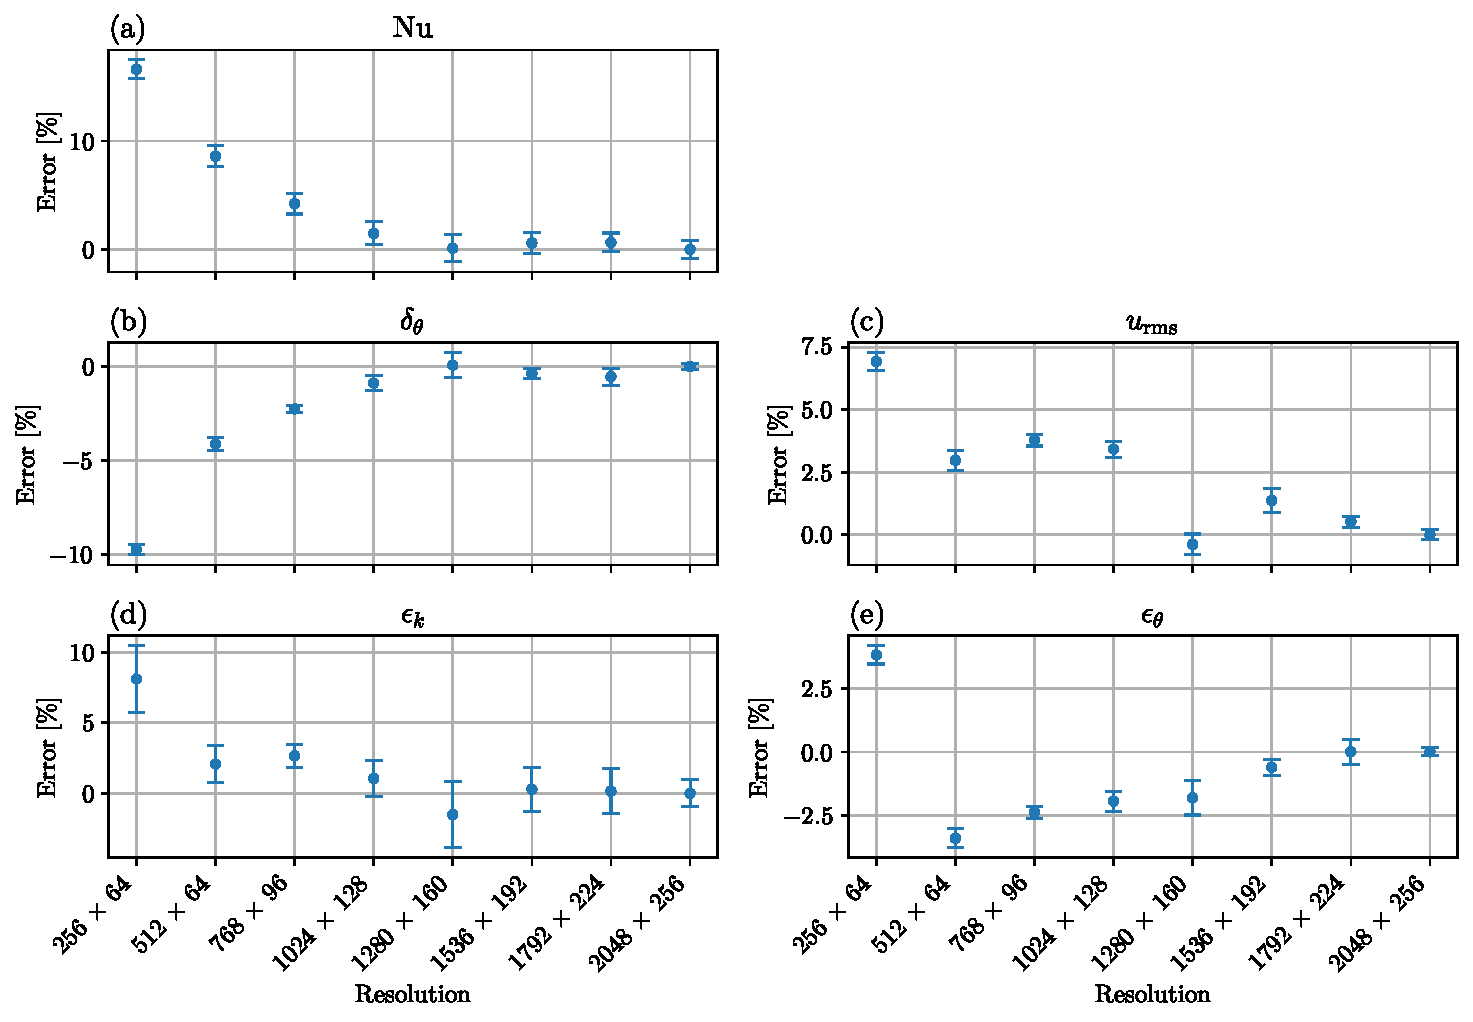
\includegraphics[width=\linewidth]{figures/resolution_dependence.pdf}
    \caption{
        Time-averaged Nusselt number \textbf{(a)}, thermal boundary layer
        thickness \textbf{(b)}, RMS speed \textbf{(c)}, kinetic energy
        dissipation rate \textbf{(d)} and thermal dissipation rate \textbf{(e)}
        as functions of model resolution, expressed as percentage errors
        relative to the values from the highest-resolution simulation ($2048
        \times 256$). Refer to the corresponding list items in the text for
        more detailed definitions of the quantities.
    }
    \label{fig:resolution_dependence}
\end{figure}


\ifSubfilesClassLoaded{%
    \emergencystretch=5em
    \printbibliography{}
}{}

\end{document}
